% Created by tikzDevice version 0.12.5 on 2024-01-22 13:11:46
% !TEX encoding = UTF-8 Unicode
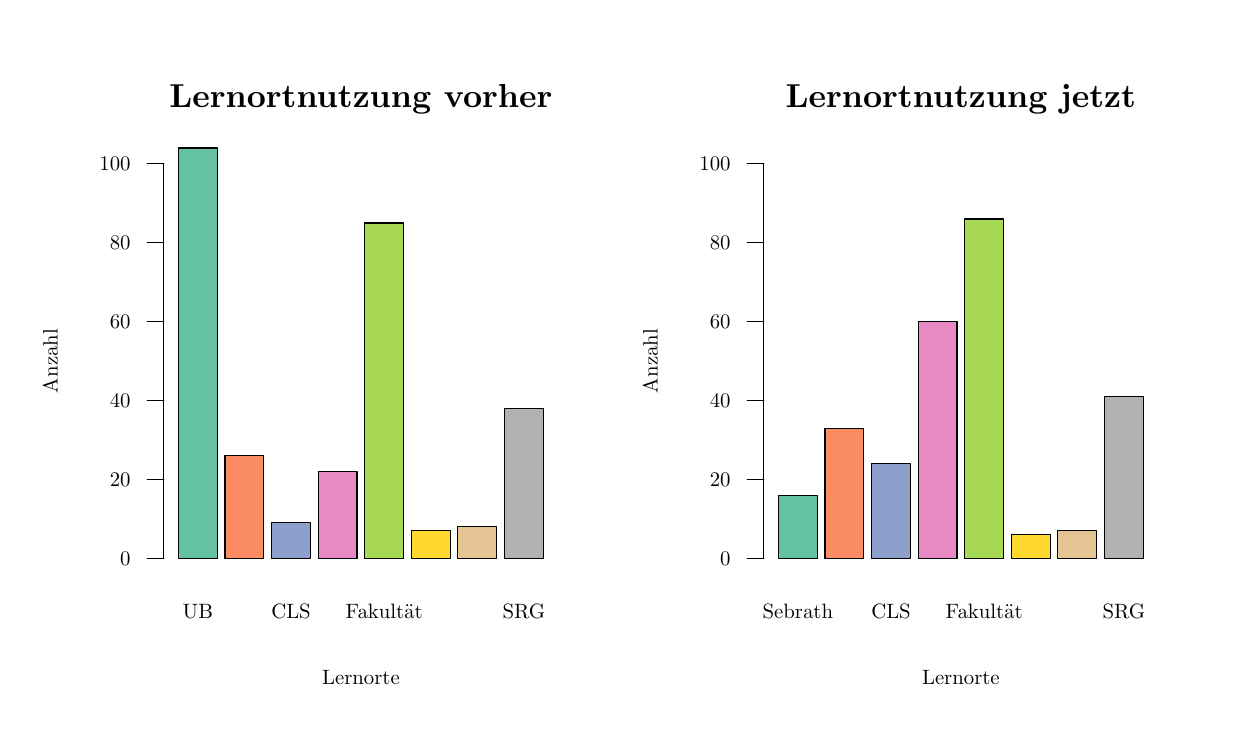
\begin{tikzpicture}[x=1pt,y=1pt]
\definecolor{fillColor}{RGB}{255,255,255}
\path[use as bounding box,fill=fillColor,fill opacity=0.00] (0,0) rectangle (433.62,252.94);
\begin{scope}
\path[clip] (  0.00,  0.00) rectangle (216.81,252.94);
\definecolor{drawColor}{RGB}{0,0,0}
\definecolor{fillColor}{RGB}{102,194,165}

\path[draw=drawColor,line width= 0.4pt,line join=round,line cap=round,fill=fillColor] ( 54.47, 61.20) rectangle ( 68.50,209.45);
\definecolor{fillColor}{RGB}{252,141,98}

\path[draw=drawColor,line width= 0.4pt,line join=round,line cap=round,fill=fillColor] ( 71.31, 61.20) rectangle ( 85.34, 98.26);
\definecolor{fillColor}{RGB}{141,160,203}

\path[draw=drawColor,line width= 0.4pt,line join=round,line cap=round,fill=fillColor] ( 88.14, 61.20) rectangle (102.17, 74.03);
\definecolor{fillColor}{RGB}{231,138,195}

\path[draw=drawColor,line width= 0.4pt,line join=round,line cap=round,fill=fillColor] (104.97, 61.20) rectangle (119.00, 92.56);
\definecolor{fillColor}{RGB}{166,216,84}

\path[draw=drawColor,line width= 0.4pt,line join=round,line cap=round,fill=fillColor] (121.81, 61.20) rectangle (135.84,182.36);
\definecolor{fillColor}{RGB}{255,217,47}

\path[draw=drawColor,line width= 0.4pt,line join=round,line cap=round,fill=fillColor] (138.64, 61.20) rectangle (152.67, 71.18);
\definecolor{fillColor}{RGB}{229,196,148}

\path[draw=drawColor,line width= 0.4pt,line join=round,line cap=round,fill=fillColor] (155.47, 61.20) rectangle (169.50, 72.60);
\definecolor{fillColor}{gray}{0.70}

\path[draw=drawColor,line width= 0.4pt,line join=round,line cap=round,fill=fillColor] (172.31, 61.20) rectangle (186.34,115.37);
\end{scope}
\begin{scope}
\path[clip] (  0.00,  0.00) rectangle (433.62,252.94);
\definecolor{drawColor}{RGB}{0,0,0}

\node[text=drawColor,anchor=base,inner sep=0pt, outer sep=0pt, scale=  0.75] at ( 61.49, 39.60) {UB};

\node[text=drawColor,anchor=base,inner sep=0pt, outer sep=0pt, scale=  0.75] at ( 95.16, 39.60) {CLS};

\node[text=drawColor,anchor=base,inner sep=0pt, outer sep=0pt, scale=  0.75] at (128.82, 39.60) {Fakultät};

\node[text=drawColor,anchor=base,inner sep=0pt, outer sep=0pt, scale=  0.75] at (179.32, 39.60) {SRG};
\end{scope}
\begin{scope}
\path[clip] (  0.00,  0.00) rectangle (216.81,252.94);
\definecolor{drawColor}{RGB}{0,0,0}

\node[text=drawColor,anchor=base,inner sep=0pt, outer sep=0pt, scale=  1.20] at (120.41,224.20) {\bfseries Lernortnutzung vorher};

\node[text=drawColor,anchor=base,inner sep=0pt, outer sep=0pt, scale=  0.75] at (120.41, 15.60) {Lernorte};

\node[text=drawColor,rotate= 90.00,anchor=base,inner sep=0pt, outer sep=0pt, scale=  0.75] at ( 10.80,132.47) {Anzahl};
\end{scope}
\begin{scope}
\path[clip] (  0.00,  0.00) rectangle (433.62,252.94);
\definecolor{drawColor}{RGB}{0,0,0}

\path[draw=drawColor,line width= 0.4pt,line join=round,line cap=round] ( 49.20, 61.20) -- ( 49.20,203.75);

\path[draw=drawColor,line width= 0.4pt,line join=round,line cap=round] ( 49.20, 61.20) -- ( 43.20, 61.20);

\path[draw=drawColor,line width= 0.4pt,line join=round,line cap=round] ( 49.20, 89.71) -- ( 43.20, 89.71);

\path[draw=drawColor,line width= 0.4pt,line join=round,line cap=round] ( 49.20,118.22) -- ( 43.20,118.22);

\path[draw=drawColor,line width= 0.4pt,line join=round,line cap=round] ( 49.20,146.73) -- ( 43.20,146.73);

\path[draw=drawColor,line width= 0.4pt,line join=round,line cap=round] ( 49.20,175.24) -- ( 43.20,175.24);

\path[draw=drawColor,line width= 0.4pt,line join=round,line cap=round] ( 49.20,203.75) -- ( 43.20,203.75);

\node[text=drawColor,anchor=base east,inner sep=0pt, outer sep=0pt, scale=  0.75] at ( 37.20, 58.62) {0};

\node[text=drawColor,anchor=base east,inner sep=0pt, outer sep=0pt, scale=  0.75] at ( 37.20, 87.13) {20};

\node[text=drawColor,anchor=base east,inner sep=0pt, outer sep=0pt, scale=  0.75] at ( 37.20,115.64) {40};

\node[text=drawColor,anchor=base east,inner sep=0pt, outer sep=0pt, scale=  0.75] at ( 37.20,144.14) {60};

\node[text=drawColor,anchor=base east,inner sep=0pt, outer sep=0pt, scale=  0.75] at ( 37.20,172.65) {80};

\node[text=drawColor,anchor=base east,inner sep=0pt, outer sep=0pt, scale=  0.75] at ( 37.20,201.16) {100};
\end{scope}
\begin{scope}
\path[clip] (216.81,  0.00) rectangle (433.62,252.94);
\definecolor{drawColor}{RGB}{0,0,0}
\definecolor{fillColor}{RGB}{102,194,165}

\path[draw=drawColor,line width= 0.4pt,line join=round,line cap=round,fill=fillColor] (271.28, 61.20) rectangle (285.31, 84.01);
\definecolor{fillColor}{RGB}{252,141,98}

\path[draw=drawColor,line width= 0.4pt,line join=round,line cap=round,fill=fillColor] (288.12, 61.20) rectangle (302.15,108.24);
\definecolor{fillColor}{RGB}{141,160,203}

\path[draw=drawColor,line width= 0.4pt,line join=round,line cap=round,fill=fillColor] (304.95, 61.20) rectangle (318.98, 95.41);
\definecolor{fillColor}{RGB}{231,138,195}

\path[draw=drawColor,line width= 0.4pt,line join=round,line cap=round,fill=fillColor] (321.78, 61.20) rectangle (335.81,146.73);
\definecolor{fillColor}{RGB}{166,216,84}

\path[draw=drawColor,line width= 0.4pt,line join=round,line cap=round,fill=fillColor] (338.62, 61.20) rectangle (352.65,183.79);
\definecolor{fillColor}{RGB}{255,217,47}

\path[draw=drawColor,line width= 0.4pt,line join=round,line cap=round,fill=fillColor] (355.45, 61.20) rectangle (369.48, 69.75);
\definecolor{fillColor}{RGB}{229,196,148}

\path[draw=drawColor,line width= 0.4pt,line join=round,line cap=round,fill=fillColor] (372.28, 61.20) rectangle (386.31, 71.18);
\definecolor{fillColor}{gray}{0.70}

\path[draw=drawColor,line width= 0.4pt,line join=round,line cap=round,fill=fillColor] (389.12, 61.20) rectangle (403.15,119.64);
\end{scope}
\begin{scope}
\path[clip] (  0.00,  0.00) rectangle (433.62,252.94);
\definecolor{drawColor}{RGB}{0,0,0}

\node[text=drawColor,anchor=base,inner sep=0pt, outer sep=0pt, scale=  0.75] at (278.30, 39.60) {Sebrath};

\node[text=drawColor,anchor=base,inner sep=0pt, outer sep=0pt, scale=  0.75] at (311.97, 39.60) {CLS};

\node[text=drawColor,anchor=base,inner sep=0pt, outer sep=0pt, scale=  0.75] at (345.63, 39.60) {Fakultät};

\node[text=drawColor,anchor=base,inner sep=0pt, outer sep=0pt, scale=  0.75] at (396.13, 39.60) {SRG};
\end{scope}
\begin{scope}
\path[clip] (216.81,  0.00) rectangle (433.62,252.94);
\definecolor{drawColor}{RGB}{0,0,0}

\node[text=drawColor,anchor=base,inner sep=0pt, outer sep=0pt, scale=  1.20] at (337.21,224.20) {\bfseries Lernortnutzung jetzt};

\node[text=drawColor,anchor=base,inner sep=0pt, outer sep=0pt, scale=  0.75] at (337.21, 15.60) {Lernorte};

\node[text=drawColor,rotate= 90.00,anchor=base,inner sep=0pt, outer sep=0pt, scale=  0.75] at (227.61,132.47) {Anzahl};
\end{scope}
\begin{scope}
\path[clip] (  0.00,  0.00) rectangle (433.62,252.94);
\definecolor{drawColor}{RGB}{0,0,0}

\path[draw=drawColor,line width= 0.4pt,line join=round,line cap=round] (266.01, 61.20) -- (266.01,203.75);

\path[draw=drawColor,line width= 0.4pt,line join=round,line cap=round] (266.01, 61.20) -- (260.01, 61.20);

\path[draw=drawColor,line width= 0.4pt,line join=round,line cap=round] (266.01, 89.71) -- (260.01, 89.71);

\path[draw=drawColor,line width= 0.4pt,line join=round,line cap=round] (266.01,118.22) -- (260.01,118.22);

\path[draw=drawColor,line width= 0.4pt,line join=round,line cap=round] (266.01,146.73) -- (260.01,146.73);

\path[draw=drawColor,line width= 0.4pt,line join=round,line cap=round] (266.01,175.24) -- (260.01,175.24);

\path[draw=drawColor,line width= 0.4pt,line join=round,line cap=round] (266.01,203.75) -- (260.01,203.75);

\node[text=drawColor,anchor=base east,inner sep=0pt, outer sep=0pt, scale=  0.75] at (254.01, 58.62) {0};

\node[text=drawColor,anchor=base east,inner sep=0pt, outer sep=0pt, scale=  0.75] at (254.01, 87.13) {20};

\node[text=drawColor,anchor=base east,inner sep=0pt, outer sep=0pt, scale=  0.75] at (254.01,115.64) {40};

\node[text=drawColor,anchor=base east,inner sep=0pt, outer sep=0pt, scale=  0.75] at (254.01,144.14) {60};

\node[text=drawColor,anchor=base east,inner sep=0pt, outer sep=0pt, scale=  0.75] at (254.01,172.65) {80};

\node[text=drawColor,anchor=base east,inner sep=0pt, outer sep=0pt, scale=  0.75] at (254.01,201.16) {100};
\end{scope}
\end{tikzpicture}
